% Báo cáo đồ án môn học cho project Kriky.
%
% Build: .\dev.ps1 report   (chạy latexmk -xelatex, xem dev.ps1)
% Đừng gọi pdflatex -- lý do ở comment đầu preamble.tex.

\documentclass[12pt,a4paper,oneside]{report}

% Preamble của báo cáo. Nạp bởi report.tex, không tự biên dịch được.
%
% BẮT BUỘC dùng XeLaTeX, không phải pdfLaTeX. Lý do nằm ở decision record trong
% docs/plans/active/2026-10-04-bao-cao-latex-plan.md: tiếng Việt cần Unicode đầy đủ và một
% font có đủ dấu tổ hợp, mà đường encoding 8-bit của pdfLaTeX vỡ ngay khi gặp một ký tự
% ngoài bảng mã.
%
% Font hệ thống mà bản build cần: Times New Roman (chữ) và Consolas (mã). Cả hai có sẵn trên
% Windows. Trên máy không có chúng, XeLaTeX sẽ dừng với lỗi "cannot find font" -- khi đó đổi
% hai dòng \setmainfont và \setmonofont bên dưới, đừng đổi gì khác.

\usepackage{fontspec}
\usepackage{polyglossia}
\setmainlanguage{vietnamese}
\setmainfont{Times New Roman}
\setmonofont{Consolas}[Scale=0.88]

\usepackage[a4paper,inner=3cm,outer=2.5cm,top=2.5cm,bottom=2.5cm]{geometry}

% polyglossia khai báo tiếng Việt là `nohyphenation`, và đúng như vậy: tiếng Việt không ngắt
% âm tiết bằng gạch nối. Hệ quả là TeX mất hẳn công cụ chính để chỉnh một dòng quá dài, nên
% văn bản tiếng Việt không nới gì sẽ đầy overfull hbox -- chữ tràn ra ngoài lề phải. Hai dòng
% dưới trả lại cho nó chỗ co giãn ở khoảng trắng giữa từ.
\setlength{\emergencystretch}{3em}
\tolerance=2000

\usepackage{graphicx}
\graphicspath{{figures/}}
% Trang ngang cho các sơ đồ dày. Kích thước bên trong \begin{landscape}, đo bằng \typeout
% chứ không suy ra: \textwidth giữ nguyên 441pt, \textheight bị gán **thành** 441pt, và thứ
% rộng 702,8pt là \linewidth. Nên bề rộng hình khổ ngang là `width=\linewidth`, còn trần
% chiều cao là `height=\textheight`. Dùng \textheight làm bề rộng -- cái tên nghe có vẻ
% đúng -- cho ra hình hẹp hơn đáng có 37%.
\usepackage{pdflscape}
\usepackage{etoolbox}           % \ifdefempty, dùng cho các dòng bìa có thể để trống
\usepackage[font=small,labelfont=bf]{caption}

\usepackage{booktabs}
\usepackage{array}
\usepackage{longtable}          % bảng 13 bảng dữ liệu ở chương 7 vắt qua trang
\usepackage{enumitem}
\setlist{nosep,leftmargin=*}

\usepackage[unicode,hidelinks]{hyperref}
\hypersetup{
  pdftitle={Kriky — Trợ lí ra đề và chữa bài},
  pdflang={vi},
}

% Một cột hẹp cố định, căn trên, dùng cho cột đầu của các bảng tra ở chương 5 và 7.
\newcolumntype{L}[1]{>{\raggedright\arraybackslash}p{#1}}


% Bốn thông tin chỉ chủ nhân báo cáo biết. Bìa in một dòng chỉ khi dòng đó có chữ, nên để
% trống vẫn build ra một bìa gọn -- không có chỗ nào hiện ra chữ "TODO".
\newcommand{\tentruong}{ĐẠI HỌC BÁCH KHOA HÀ NỘI}
\newcommand{\tenkhoa}{}
\newcommand{\tenmonhoc}{}
\newcommand{\tengiangvien}{}

\newcommand{\tentacgia}{biabeogo147}
\newcommand{\linkrepo}{https://github.com/biabeogo147/AI-Assessment-and-Feedback-Assistant}

% In một dòng bìa, và bỏ qua nếu nội dung rỗng.
%
% Dùng \ifdefempty của etoolbox chứ không phải phép thử `\ifx\relax#2\relax` quen thuộc: ở
% đây #2 luôn là **một macro** như \tengiangvien, nên phép thử ấy so chính cái token đó với
% \relax, thấy khác, và in dòng ra kể cả khi macro rỗng. Lỗi ấy đã xảy ra thật -- bìa in
% "Giảng viên hướng dẫn:" treo lơ lửng không có tên -- và chỉ lộ ra khi nhìn trang in.
% Nhóm \begingroup...\endgroup là bắt buộc, không phải thói quen: tham số thứ ba của
% \ifdefempty chạy **không có nhóm**, nên một \bfseries hay \scshape truyền vào #1 sẽ rò ra
% và nhuộm hết phần bìa còn lại. Đã xảy ra thật: cả tên đề tài lẫn ngày tháng cùng hoá đậm.
\newcommand{\dongbia}[2]{%
  \ifdefempty{#2}{}{\begingroup#1#2\par\endgroup}%
}

\begin{document}

% polyglossia dịch sẵn phần lớn nhãn, nhưng nó gọi hai danh mục là "Danh sách". Quy ước của
% một đồ án tiếng Việt là "Danh mục", nên sửa ở đây -- sau \begin{document}, vì polyglossia
% nạp bộ nhãn của nó lúc tài liệu bắt đầu và sẽ ghi đè một \renewcommand đặt trong preamble.
\renewcommand{\listfigurename}{Danh mục hình vẽ}
\renewcommand{\listtablename}{Danh mục bảng}

\begin{titlepage}
\centering
\vspace*{0.5cm}


\includegraphics[height=3.2cm]{Logo_DHBK_HN.png}\par
\vspace{0.6cm}

\dongbia{\large\bfseries}{\tentruong}
\dongbia{\large}{\tenkhoa}

\vfill

{\scshape\large Báo cáo đồ án môn học\par}
\vspace{0.4cm}
\dongbia{\large}{\tenmonhoc}

\vspace{1.6cm}
{\Huge\bfseries Kriky\par}
\vspace{0.6cm}
{\LARGE Trợ lí ra đề và chữa bài\par}
\vspace{0.4cm}
{\large Ý tưởng, luồng nghiệp vụ và kiến trúc\par}

\vfill

{\large Tác giả: \tentacgia\par}
\dongbia{\large Giảng viên hướng dẫn: }{\tengiangvien}

\vspace{0.8cm}
{\small Mã nguồn: \url{\linkrepo}\par}

\vspace{0.6cm}
{\large\today\par}

\end{titlepage}

\tableofcontents
\listoffigures
\listoftables

\chapter{Đặt vấn đề}
\label{ch:dat-van-de}

\section{Bối cảnh}

Ở trường phổ thông, một bài kiểm tra thường kết thúc khi giáo viên trả điểm. Học sinh nhận lại bài,
nhìn những câu bị gạch chéo, rồi phần lớn dừng ở đó. Thứ thực sự làm thay đổi kết quả học tập là
việc hiểu ra mình sai ở đâu và làm lại được, nhưng việc đó hiếm khi xảy ra, vì nó cần một cuộc trao
đổi riêng cho từng em về từng câu.

Giáo viên không phải không muốn làm. Vấn đề nằm ở khối lượng công việc. Một lớp bốn mươi học sinh
làm một đề mười câu sẽ sinh ra bốn trăm lượt trả lời, và mỗi lượt sai có thể sai vì một lý do khác
nhau. Giải thích riêng cho từng em, rồi ra thêm một câu tương tự để kiểm xem em đã sửa được chưa, là
công việc tăng theo sĩ số và không có cách nào rút gọn.

Kriky là hệ thống được xây để gánh phần công việc đó, nhưng không lấy đi quyền quyết định của giáo
viên. Hình~\ref{fig:domain-context} cho thấy ranh giới của hệ thống: hai actor ở hai phía, cùng
những gì đi vào và đi ra.

\begin{landscape}
\begin{figure}[p]
  \centering
  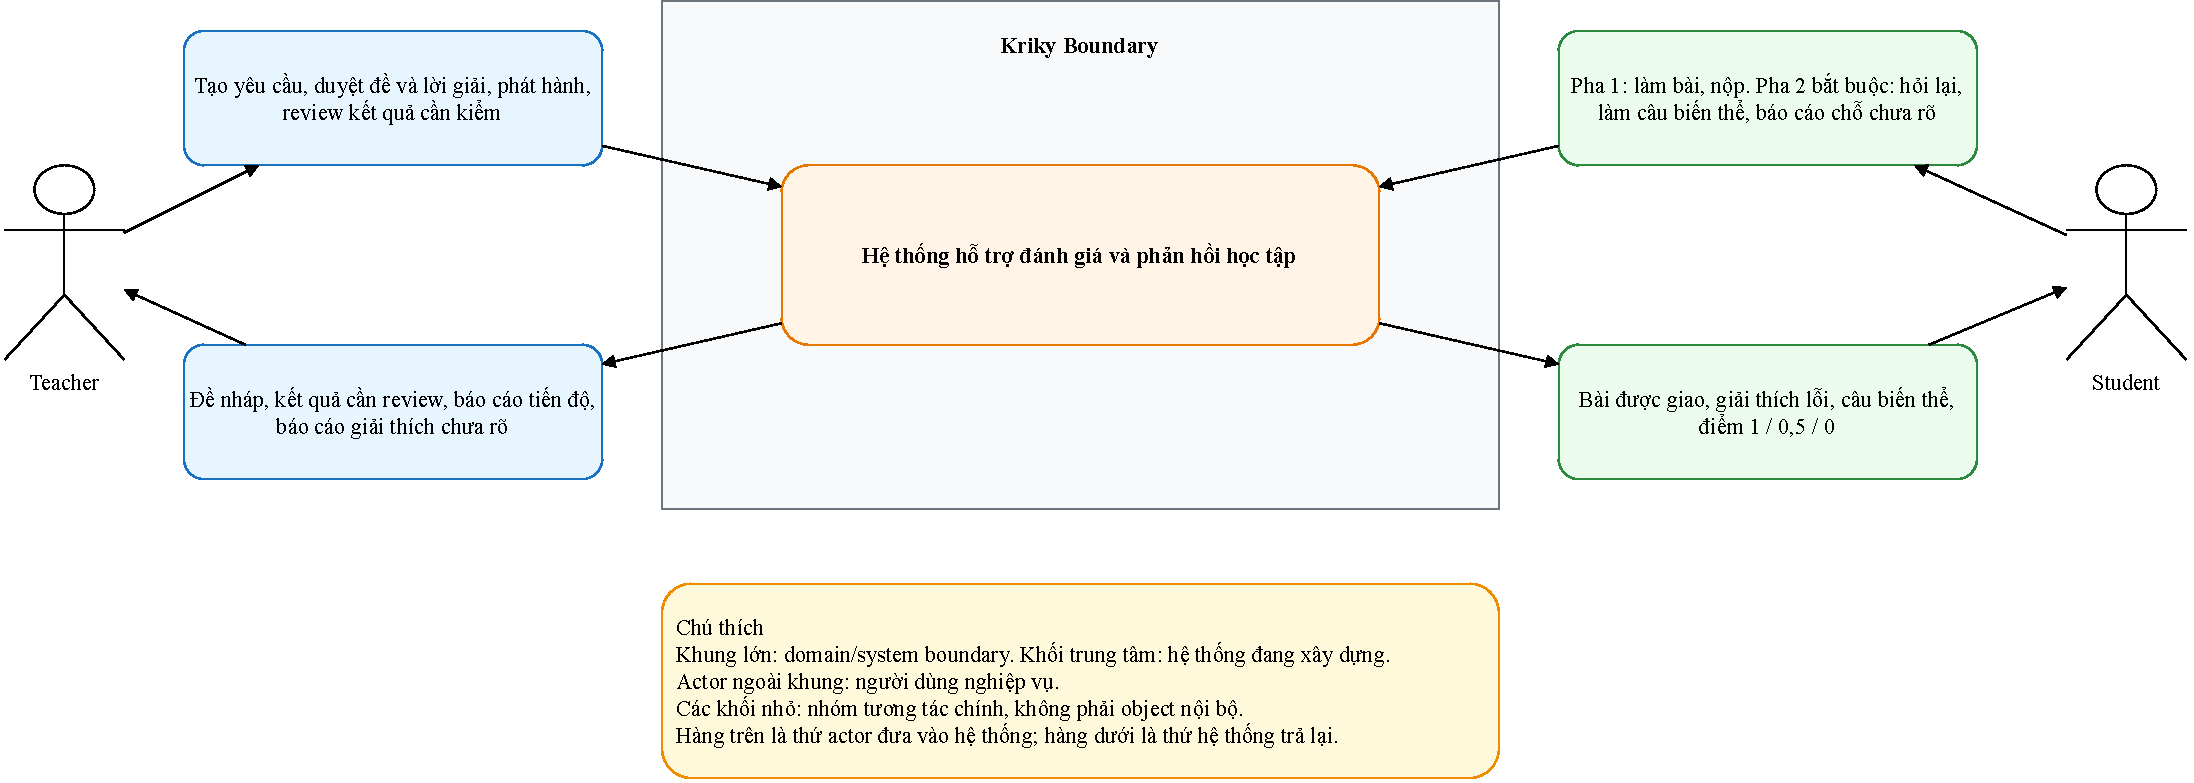
\includegraphics[width=\linewidth,height=\textheight,keepaspectratio]{domain-context.pdf}
  \caption[Domain Context]{Domain Context --- ranh giới hệ thống, hai actor, và những gì đi qua
  ranh giới ấy}
  \label{fig:domain-context}
\end{figure}
\end{landscape}

\section{Vấn đề cần giải quyết}

Phần tốn thời gian nhất của giáo viên không phải là gõ ra đề bài, mà là năm việc sau. Cả năm đều là
công việc chuyên môn:

\begin{itemize}
  \item Soạn đề bám đúng mục tiêu học tập, thay vì gom câu hỏi cho đủ số lượng.
  \item Tạo phương án nhiễu có ý nghĩa. Một phương án sai ngẫu nhiên không nói lên điều gì, còn
        một phương án nhiễu tốt là phương án mà học sinh mắc một lỗi cụ thể sẽ chọn.
  \item Chấm bài và viết nhận xét cho từng học sinh.
  \item Phân định học sinh sai vì thiếu kiến thức, vì suy luận hỏng, vì tính nhầm, hay vì hiểu
        sai một khái niệm.
  \item Ra câu biến thể của đúng câu học sinh vừa làm sai, để kiểm xem em đã sửa được chỗ sai đó
        hay chỉ nhớ được đáp án.
\end{itemize}

Phía học sinh, nhu cầu ngược lại nhưng khớp vào: phản hồi cần đến nhanh, và bài luyện tập cần đúng
với điểm yếu của riêng mình. Một phản hồi đúng nhưng đến sau hai tuần thì không còn tác dụng, vì học
sinh đã quên mình nghĩ gì lúc làm bài.

\section{Mục tiêu sản phẩm}

Hệ thống hướng tới bốn mục tiêu nghiệp vụ:

\begin{enumerate}
  \item Hỗ trợ giáo viên tạo đề từ một yêu cầu bằng ngôn ngữ tự nhiên. Một đề có hai nguồn câu
        hỏi: nội dung sinh mới, và kho câu hỏi đã dùng qua.
  \item Hỗ trợ chấm bài và sinh nhận xét có căn cứ. Mỗi nhận xét phải dẫn được về một bằng
        chứng, thay vì là một lời khuyên chung chung.
  \item Phân tích lỗi sai hoặc hiểu nhầm khái niệm của học sinh.
  \item Bắt buộc học sinh chữa lại những câu đã sai, ngay trong cùng bài kiểm tra.
\end{enumerate}

Mục tiêu thứ tư là thứ phân biệt hệ thống này với một công cụ sinh đề thông thường.
Chương~\ref{ch:y-tuong} dành phần lớn dung lượng cho nó.

\section{Phạm vi}

Hệ thống dựng trọn một vòng nghiệp vụ, thay vì dựng sâu một khâu:

\begin{itemize}
  \item Giáo viên tạo, xem lại và phát hành đề. Việc duyệt bao gồm cả lời giải và ánh xạ từ
        phương án nhiễu sang lỗi, không chỉ câu hỏi và đáp án.
  \item Giai đoạn 2: Học sinh làm bài và nộp bài.
  \item Hệ thống chấm bài và tra lỗi sai từ phương án nhiễu mà học sinh đã chọn.
  \item Kết quả có độ tin cậy thấp, hoặc có dấu hiệu bất thường, đi vào hàng đợi chờ giáo viên
        xem lại.
  \item Giai đoạn 2: hệ thống giải thích lỗi và sinh câu biến thể, học sinh làm lại cho tới khi điểm
        của từng câu được chốt.
\end{itemize}

\chapter{Ý tưởng sản phẩm}
\label{ch:y-tuong}

Dùng AI để sinh đề là chuyện đã có nhiều người làm. Chương này nói về những chỗ Kriky quyết khác, và
lý do đằng sau mỗi quyết định.

\section{Luồng tổng thể}
\label{sec:vong-hoc}

Ý tưởng lõi không nằm ở việc sinh câu hỏi, mà ở việc khép kín một vòng tám bước:

\begin{enumerate}
  \item Giáo viên tạo và duyệt đề.
  \item Học sinh làm bài.
  \item Hệ thống đánh giá đáp án và cách tư duy.
  \item Hệ thống xác định lỗi sai hoặc hiểu nhầm khái niệm.
  \item Hệ thống giải thích lỗi, học sinh hỏi lại đến khi hiểu.
  \item Hệ thống tạo câu biến thể của chính câu vừa sai.
  \item Học sinh làm lại, tối đa ba vòng cho mỗi câu.
  \item Mỗi câu chốt ở một trong ba mức điểm, và bài kết thúc.
\end{enumerate}

Hình~\ref{fig:vong-hoc} vẽ tám bước ấy kèm chỗ vòng lặp quay lại, và nó là bản đồ của cả chương
này.

\begin{landscape}
\begin{figure}[p]
  \centering
  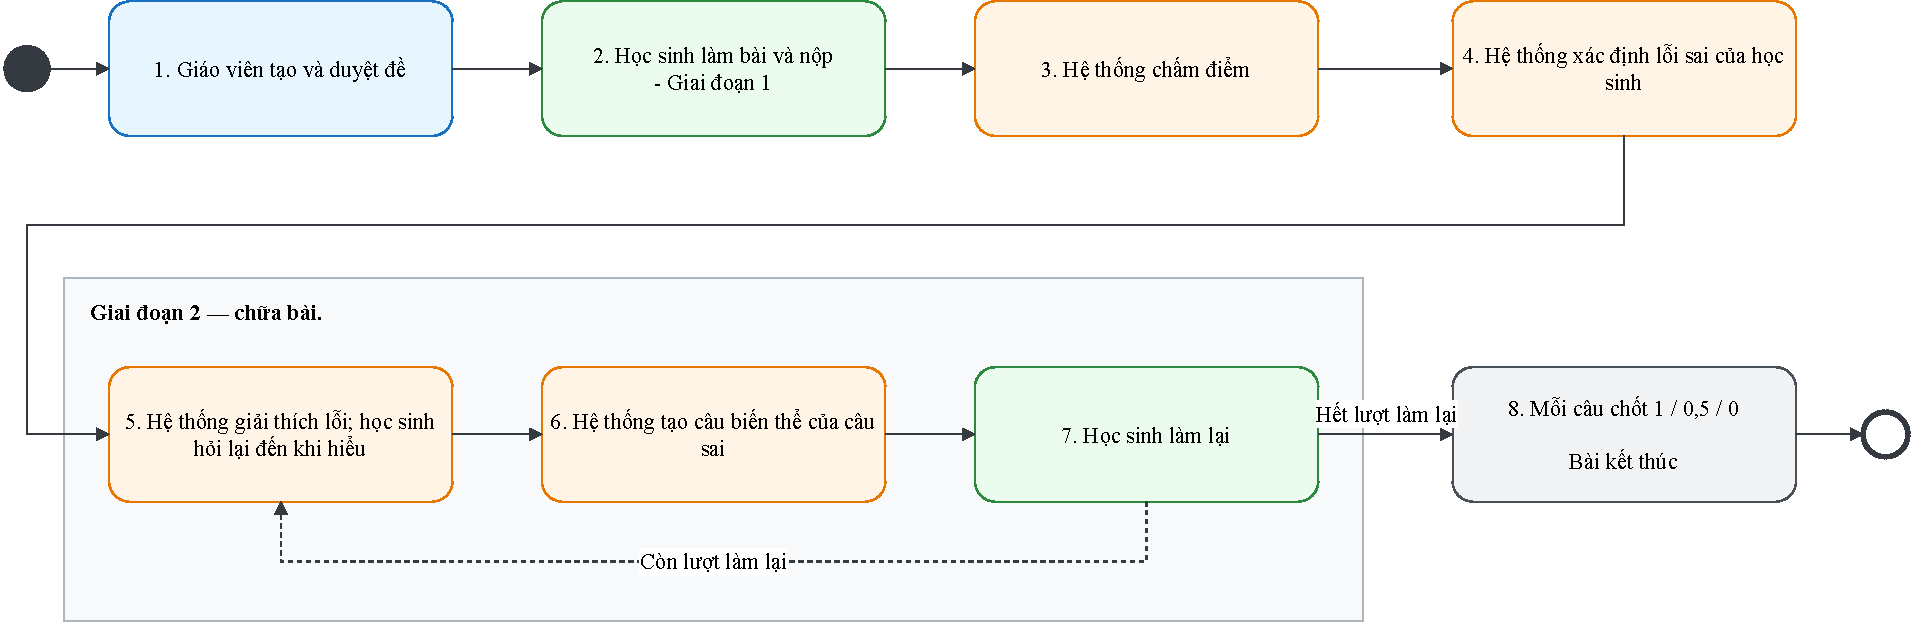
\includegraphics[width=\linewidth,height=\textheight,keepaspectratio]{vong-hoc.pdf}
  \caption[Vòng học khép kín]{Vòng học khép kín --- tám bước, và chỗ vòng lặp quay lại}
  \label{fig:vong-hoc}
\end{figure}
\end{landscape}

\section{Hai giai đoạn làm bài của học sinh}
\label{sec:hai-giai-doan}

\emph{Bước 2, 7 và 8 của hình~\ref{fig:vong-hoc}.}

Một bài kiểm tra có hai giai đoạn: giai đoạn 1 là làm bài và nộp, 
giai đoạn 2 là chữa những câu đã sai. Nộp bài kết thúc giai đoạn 1 chứ không kết thúc
bài. Bài chỉ kết thúc khi giai đoạn 2 xong, hoặc khi hạn của giai đoạn 2 hết.

Kéo theo đó là một hệ quả cần nói rõ: một bài kiểm tra có hai trạng thái hoàn thành khác nhau,
\emph{đã nộp} và \emph{đã hoàn thành}, và chúng không thay thế cho nhau được.

\section{Làm sao phân tích lỗi của học sinh?}
\label{sec:nhan-loi}

\emph{Bước 4 của hình~\ref{fig:vong-hoc}.}

Với hình thức trắc nghiệm, việc chấm chỉ là một phép so. Khó khăn nằm ở chẩn đoán lỗi sai của học sinh, 
bởi cùng chọn một phương án sai có thể do nhiều lỗi khác nhau sinh ra. Nếu hệ thống đoán lỗi rồi đi giải 
thích một lỗi học sinh không hề mắc thì nó còn tệ hơn im lặng: em vừa mất thời gian, vừa được dạy sai chỗ.

Vì vậy, mỗi phương án sai phải mang theo lỗi mà nó đại diện, và được soạn cùng câu hỏi
chứ không suy ra lúc chấm. 

Hai luật đi kèm:

\begin{itemize}
  \item Mỗi câu hỏi phải mang theo lời giải có nhiều hơn một cách làm. 
  \item Số phương án không cố định. Một câu có thể có ba, bốn hay năm lựa chọn tuỳ từng câu,
        nhưng chỉ đúng một lựa chọn là đáp án đúng. Mọi phương án còn lại đều là nhiễu, nên đều
        phải có lỗi gắn kèm.
\end{itemize}

\section{Tạo câu hỏi mới dựa trên câu làm sai}
\label{sec:ba-vong}

\emph{Bước 6 và 7 của hình~\ref{fig:vong-hoc}}

Khi học sinh sai câu 3, hệ thống sinh câu 3\`, gọi là câu biến thể. Thứ cần chữa là một lỗi cụ thể vừa xảy ra, không phải một chủ đề.

Câu biến thể giữ nguyên dạng đề và cách làm, chỉ đổi dữ kiện, con số và cách hỏi. Đó là cách duy
nhất kiểm được rằng học sinh đã sửa đúng chỗ mình sai, chứ không phải chỉ nhớ được đáp án.

\section{Thang điểm}
\label{sec:thang-diem}

\emph{Bước 8 của hình~\ref{fig:vong-hoc}.}

\begin{table}[htbp]
\centering
\caption{Ba mức điểm của một câu hỏi}
\label{tab:thang-ba-muc}
\begin{tabular}{@{}cl@{}}
\toprule
\textbf{Điểm} & \textbf{Nghĩa} \\
\midrule
1   & Đúng ngay ở giai đoạn 1 \\
0,5 & Sai ở giai đoạn 1 nhưng chữa được ở giai đoạn 2 \\
0   & Sai và không chữa được \\
\bottomrule
\end{tabular}
\end{table}

Ba mức thay vì hai, vì hai mức sẽ biến việc chữa bài thành công việc không được có ý nghĩa. Một học
sinh sửa được lỗi của mình đã học đúng thứ mà bài kiểm tra muốn dạy, và mức giữa là chỗ duy nhất ghi
nhận điều đó. Vì vậy giai đoạn 2 chỉ cộng chứ không bao giờ trừ: điểm tính ngay sau khi nộp là sàn.

\section{Giáo viên đưa ra quyết định ở đâu?}
\label{sec:ba-cong}

\emph{Bước 1 của hình~\ref{fig:vong-hoc}.}

Với nội dung đề, trợ lí viết còn giáo viên quyết nội dung đó có đến tay học sinh hay không. 
Giáo viên bắt buộc tham gia ở ba điểm, hai ở đầu ra và một ở đầu vào:

\begin{enumerate}
  \item Duyệt đề trước khi phát hành (đầu ra).
  \item Trợ lí hỏi lại khi chưa đủ thông tin, thay vì tự đoán (đầu vào).
\end{enumerate}

\chapter{Actor và khái niệm nghiệp vụ}
\label{ch:actor-va-khai-niem}

\section{Hai actor}

Hệ thống có đúng hai actor nghiệp vụ: \textbf{Teacher} và \textbf{Student}.

\subsection{Teacher}

Teacher là người đưa ra các quyết định. Teacher có thể:

\begin{itemize}
  \item Nhập yêu cầu tạo đề.
  \item Xem và chỉnh sửa đề do trợ lí tạo.
  \item Duyệt đề trước khi phát hành.
  \item Phát hành đề cho một hoặc nhiều lớp.
  \item Xem kết quả làm bài của học sinh.
  \item Xem báo cáo học sinh gửi về chỗ trợ lí giải thích chưa rõ.
\end{itemize}

\subsection{Student}

Student là người nhận đề, làm bài và luyện tập. Student có thể:

\begin{itemize}
  \item Xem bài kiểm tra được giao.
  \item Chọn đáp án và nộp bài (giai đoạn 1).
  \item Nghe giải thích lỗi và hỏi lại đến khi hiểu (giai đoạn 2).
  \item Làm câu biến thể của những câu đã sai (giai đoạn 2).
  \item Báo cáo chỗ trợ lí giải thích chưa rõ.
\end{itemize}

\section{Từ điển khái niệm}
\label{sec:tu-dien}

\begin{itemize}
  \item \textbf{Assessment}: Bài kiểm tra, hay bộ câu hỏi được giao cho học sinh.
  \item \textbf{Question}: Câu hỏi trong một assessment.
  \item \textbf{Distractor}: Phương án sai \emph{có chủ đích}, đại diện cho một lỗi hoặc một hiểu nhầm cụ
        thể. Không phải đáp án nhiễu ngẫu nhiên.
  \item \textbf{Submission}: Việc nộp bài, và là mốc kết thúc \emph{giai đoạn 1} --- không phải
        mốc kết thúc bài kiểm tra.
  \item \textbf{Attempt}: Cả một lần làm bài của một học sinh trên một đề, trải qua \textbf{cả hai giai
        đoạn}. Mỗi học sinh có \emph{nhiều nhất} một Attempt cho mỗi đề --- em chưa vào làm thì
        không có Attempt nào. Nó xong khi mọi câu sai đã chốt, hoặc khi hạn giai đoạn 2 đi qua.
  \item \textbf{Feedback}: Phản hồi / nhận xét của trợ lí cho những thắc mắc của học sinh.
  \item \textbf{Misconception}: Hiểu nhầm khái niệm, hoặc lỗi sai có tính lặp lại.
  \item \textbf{Mastery}: Mức độ thành thạo của học sinh với một mục tiêu học tập. Khái niệm này vẫn còn
        trong từ điển nhưng \textbf{không còn quyết định gì} --- điều kiện dừng của vòng chữa bài
        là số vòng, không phải mastery.
  \item \textbf{Giai đoạn 1}: Phần làm bài và nộp.
  \item \textbf{Giai đoạn 2}: Phần chữa bài.
  \item \textbf{Lượt}: Một lượt cho phép học sinh làm lại các câu sai của giai đoạn trước / lượt trước.
  \item \textbf{Câu biến thể}: Câu sinh từ \emph{câu học sinh làm sai ở giai đoạn 1}: giữ cấu trúc và lỗi cần
        kiểm, chỉ đổi dữ kiện.
  \item \textbf{Lời giải}: Cách làm đi kèm mỗi câu hỏi, bắt buộc có nhiều hơn một cách. Trợ lí
        dựa vào lời giải để giải thích cho học sinh.
  \item \textbf{Class}: Lớp học có sẵn danh sách học sinh. Giáo viên tạo lớp. Phát hành đề phải
        chọn một lớp đã tạo từ trước.
  \item \textbf{Question Bank}: Ngân hàng đề.
  \item \textbf{Document}: Tài liệu PDF của giáo viên, nằm trong kho lưu trữ riêng của từng tài
        khoản. Cung cấp kiến thức và giới hạn phạm vi ra đề.
  \item \textbf{Scope}: Phạm vi ra đề, chương và khoảng trang trong một \emph{Document}.
  \item \textbf{Service}: Một đơn vị chạy độc lập trong hệ thống. Có năm: \texttt{frontend},
        \texttt{backend}, \texttt{agent}, \texttt{document}, \texttt{ingest}.
  \item \textbf{Job} và \textbf{Task}: Hai thứ khác nhau. Một \emph{task} là \emph{tên} của một loại
        việc. Một \emph{job} là một lần chạy của task ấy, có id riêng và có thể thất bại riêng.
  \item \textbf{Queue}: Nơi một service đẩy job vào và một service khác lấy ra làm. Job nằm lại
        trên queue đến khi có ai lấy, nên tắt máy giữa chừng không mất việc.
  \item \textbf{Worker}: Tiến trình ngồi nghe một queue, lấy job xuống và chạy. Nó không nhận lời
        gọi từ ngoài; thứ duy nhất nó đọc là queue.
  \item \textbf{Pub/sub}: Phát một tiếng lên một \emph{channel}: ai đang nghe thì nhận, ai không
        nghe thì mất. Khác queue ở chỗ nó \textbf{không giữ lịch sử} và không chở nội dung --- nó
        chỉ nói \emph{có cái gì vừa đổi}, còn muốn biết đổi gì thì phải đi hỏi lại.
  \item \textbf{SSE} và \textbf{Polling}: Hai cách để màn hình biết có thứ mới. Với \emph{SSE},
        \texttt{backend} giữ một kết nối mở và \emph{hích} xuống mỗi khi có gì đổi. Với \emph{polling},
        màn hình tự hỏi lại theo một chu kì. Hệ thống dùng \emph{SSE}; \emph{polling} là phương án
        nó \textbf{không} dùng, và có trong từ điển để gọi tên thứ đã bị bỏ.
  \item \textbf{Gateway}: Cửa duy nhất đi vào một vùng. \texttt{backend} là gateway của cả hệ thống:
        không màn hình nào gọi thẳng \texttt{agent}, \texttt{document} hay \texttt{ingest}.
  \item \textbf{Store}: Ba kho của hệ thống là ba loại khác nhau, không nên gọi chung một chữ:
        \emph{database} giữ dữ liệu có cấu trúc, \emph{object store} (một \emph{bucket}) giữ byte
        của tệp, và \emph{queue} giữ job đang chờ.
  \item \textbf{Draft}: Đề đang soạn, chưa duyệt. Câu hỏi ở trạng thái này sửa và xoá được tự do.
  \item \textbf{Approve}: Chốt rằng đề đã dùng được. Đây là một \emph{trạng thái}, không phải một
        thao tác: nó có cả cạnh ngược (\emph{unapprove}), và chỉ đề đã approve mới phát hành được.
  \item \textbf{Publish} và \textbf{Publication}: \emph{Publish} là phát hành một đề cho một lớp. Một
        \emph{Publication} là bản ghi sinh ra từ việc đó: một lớp đã chọn, cộng năm thứ giáo viên
        đặt cho lớp đó.
        Cùng một đề phát hành cho hai lớp là hai \emph{Publication}.
  \item \textbf{Mark} và \textbf{Score}: \emph{Mark} là điểm của \emph{một câu}; \emph{score} là điểm
        của \emph{cả bài}. Tiếng Việt gọi cả hai là ``điểm'', nên báo cáo giữ hai chữ tiếng Anh ở
        những chỗ cần phân biệt.
  \item \textbf{opens\_at} / \textbf{closes\_at} / \textbf{remediation\_deadline}: Ba mốc thời
        gian của một \emph{Publication}. Hai mốc đầu mở và đóng giai đoạn 1; mốc thứ ba là hạn
        của giai đoạn 2. Chữ ``hạn'' một mình không nói rõ là hạn nào.
  \item \textbf{Tool}: Một việc có tên mà \texttt{agent} được phép \emph{đề xuất} chạy, kèm tham
        số. Danh sách tool là một \textbf{ràng buộc}, không phải một tiện ích: duyệt đề và phát
        hành đề cố ý không có tool nào, nên \texttt{agent} không có đường nào để đề xuất chúng.
\end{itemize}

\chapter{Các luồng nghiệp vụ}
\label{ch:luong-nghiep-vu}

Nghiệp vụ của hệ thống gồm năm luồng. 
Hình~\ref{fig:activity-overview} và hình~\ref{fig:vong-hoc} mô tả cùng một luồng, nhưng ở hai mức chi tiết khác nhau. 

\begin{landscape}
\begin{figure}[p]
  \centering
  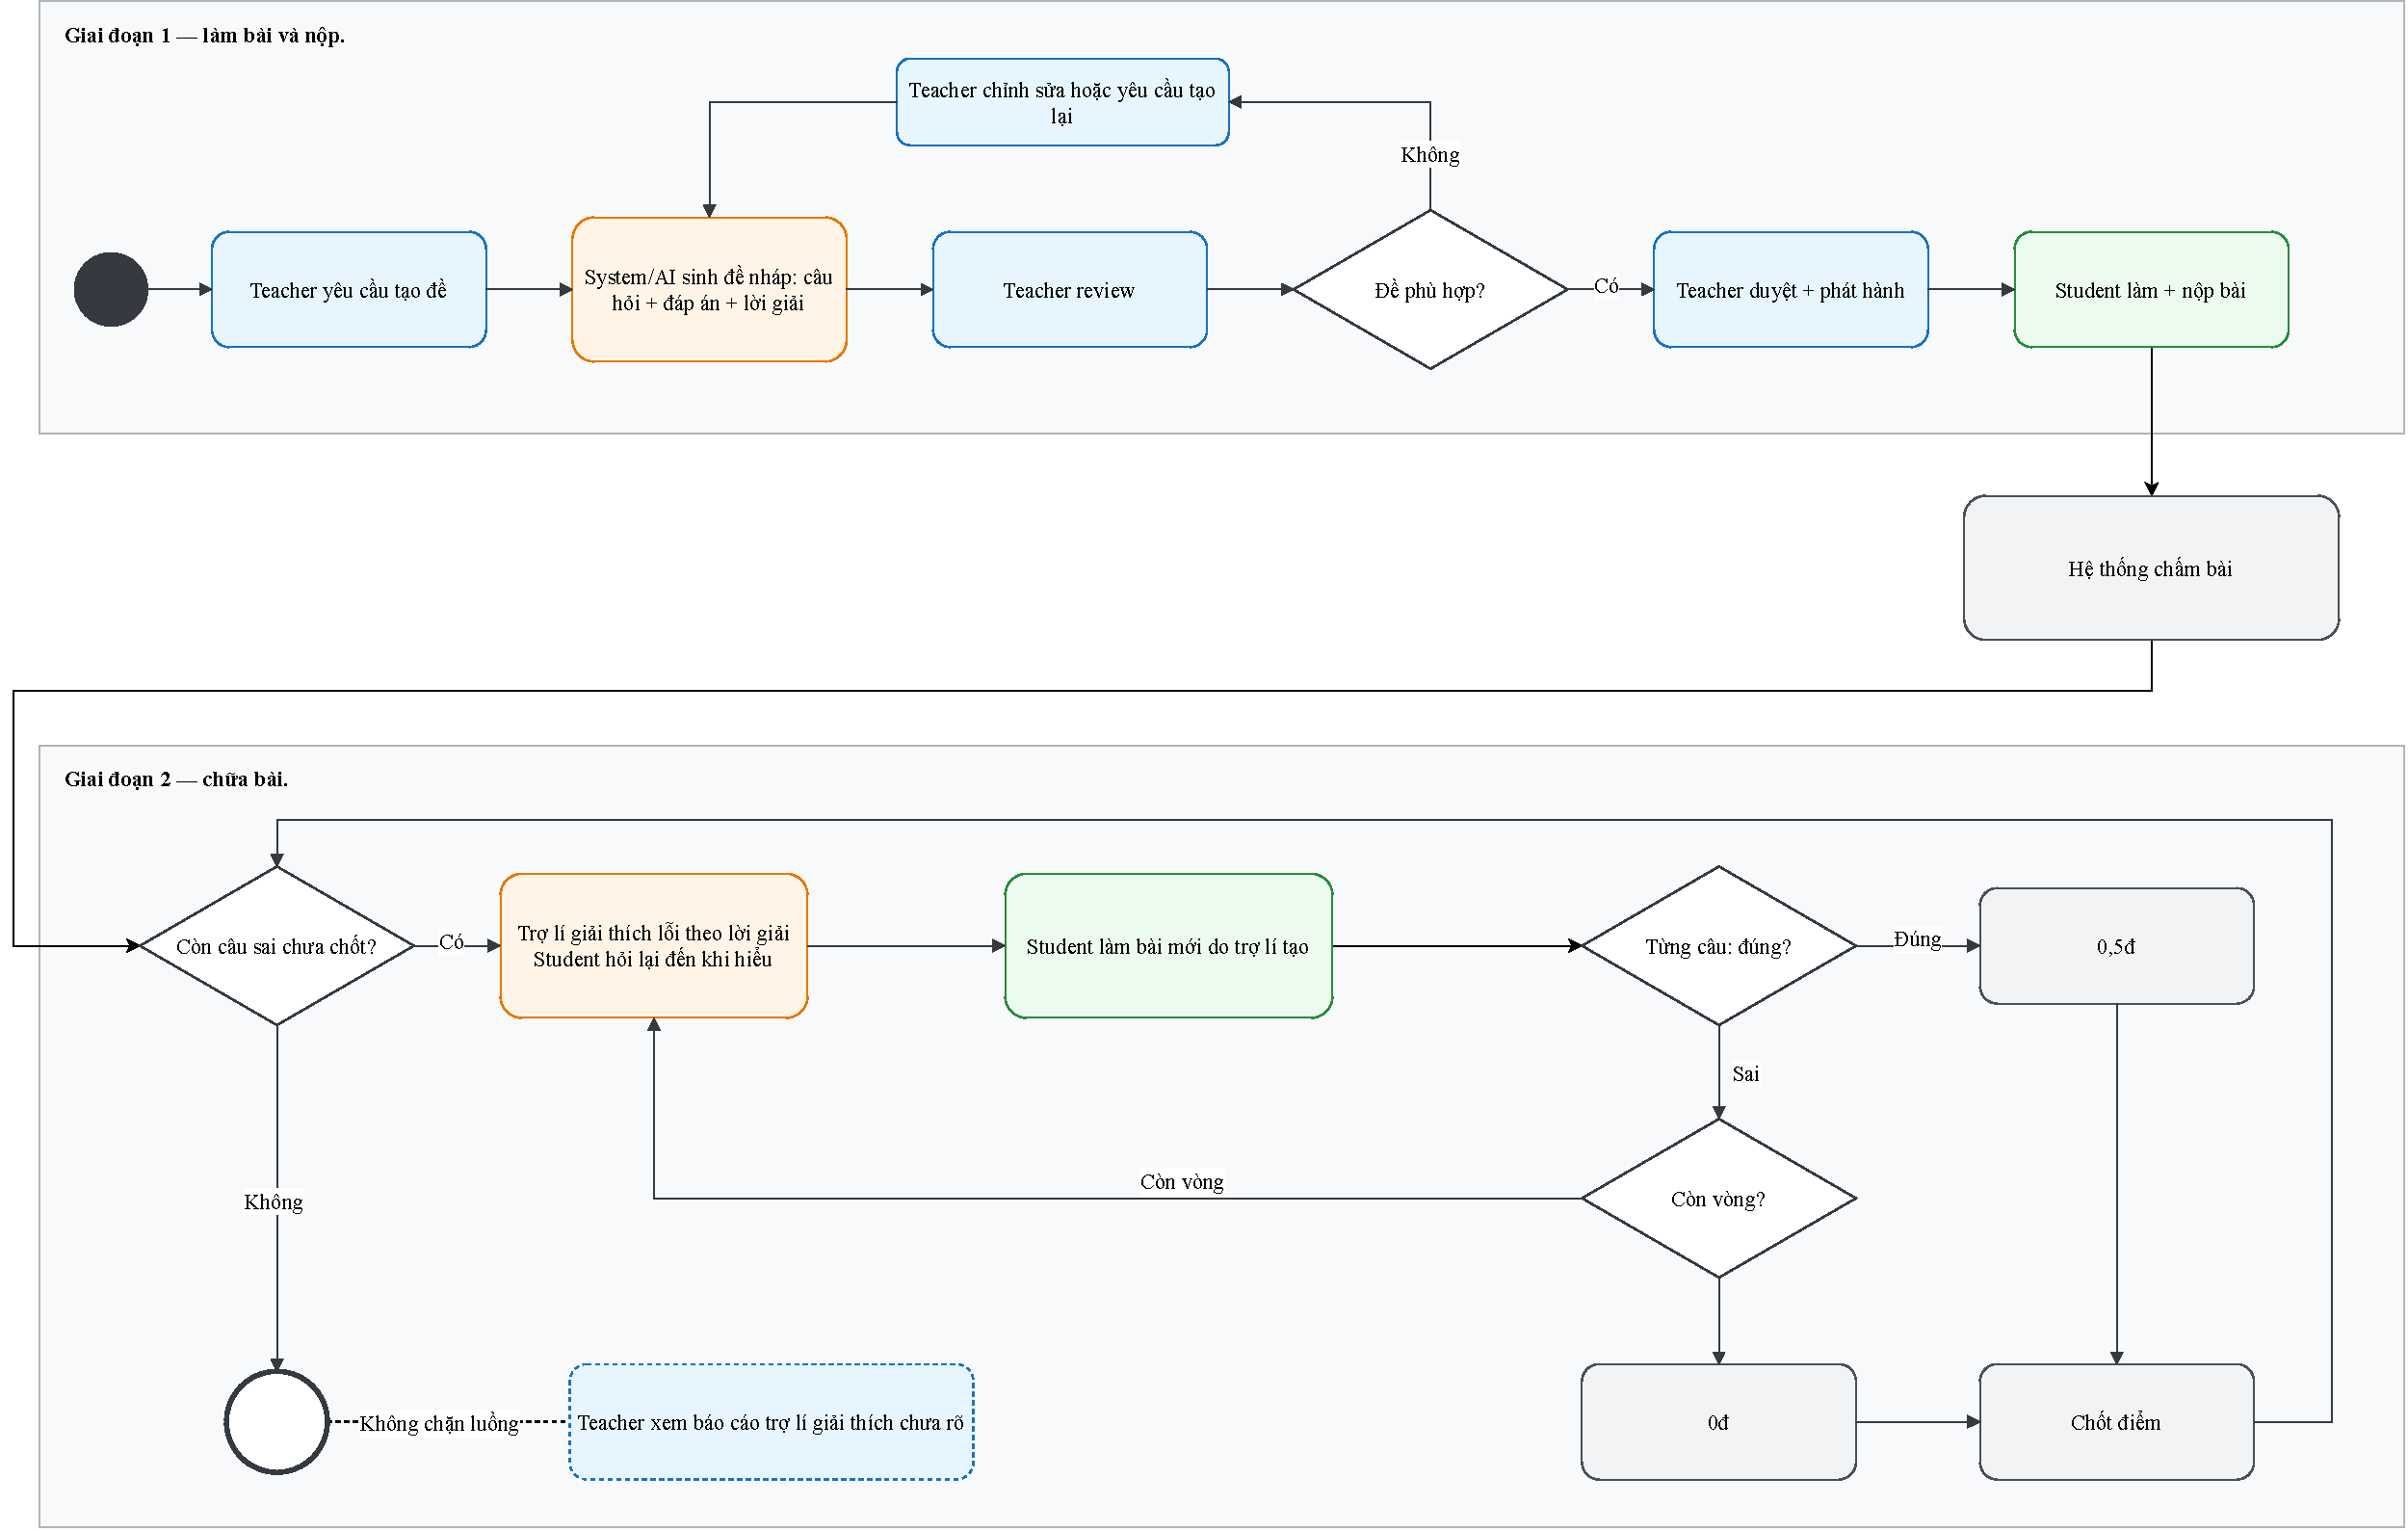
\includegraphics[width=\linewidth,height=\textheight,keepaspectratio]{activity-overview.pdf}
  \caption[Activity Overview]{Activity Overview --- toàn bộ vòng, hai giai đoạn nằm trong hai khung
  riêng}
  \label{fig:activity-overview}
\end{figure}
\end{landscape}

\section{Workflow 1 --- Tạo và duyệt đề}

\paragraph{Mục tiêu.} Giúp giáo viên tạo được đề phù hợp với mục tiêu học tập, nhưng giáo viên
vẫn là người duyệt cuối cùng trước khi phát hành.

\paragraph{Luồng chính.}
\begin{enumerate}
  \item Teacher nhập yêu cầu tạo đề.
  \item Teacher cung cấp ràng buộc: chủ đề, độ khó, số lượng câu hỏi, loại bài kiểm tra, thời
        gian làm bài.
  \item \texttt{System/AI} phân tích yêu cầu.
  \item \texttt{System/AI} tạo đề nháp gồm câu hỏi, phương án trả lời, đáp án đúng, lời giải và
        metadata cơ bản.
  \item Teacher xem đề nháp.
  \item Teacher chỉnh sửa thủ công, hoặc yêu cầu tạo lại một phần.
  \item Teacher duyệt đề.
  \item Teacher phát hành đề cho Student.
\end{enumerate}

\paragraph{Điểm kiểm soát.} Teacher phải duyệt đề trước khi đề được phát hành. Đề kiểm tra ảnh
hưởng trực tiếp đến việc đánh giá học sinh, nên trợ lí không được tự phát hành.

\section{Workflow 2 --- Làm bài (giai đoạn 1)}

\paragraph{Mục tiêu.} Cho phép học sinh làm bài và ghi nhận bài nộp để hệ thống đánh giá.

\paragraph{Luồng chính.}
\begin{enumerate}
  \item Student nhận assessment đã được Teacher phát hành.
  \item Student vào làm, \emph{tới hết} giờ đóng.
  \item Student trả lời câu hỏi trắc nghiệm.
  \item Student nộp bài.
  \item Hệ thống ghi nhận submission để đánh giá.
\end{enumerate}

\subsection{Ba mốc thời gian}
\label{sec:ba-con-so}

Giai đoạn 1 có ba tham số thời gian độc lập: thời gian làm bài, giờ mở và giờ đóng.

Luật là: giờ đóng chặn việc \emph{vào làm}, không chặn việc nộp. Học sinh vào tới hết giờ đóng vẫn
được. Ai đã vào rồi thì không bị dừng giữa chừng, và được đủ thời gian làm bài kể cả khi tràn qua giờ đóng.
Ví dụ, đóng lúc 18:00 với thời gian làm bài 15 phút thì bài cuối có thể nộp lúc 18:15.

\section{Workflow 3 --- Chấm bài và sinh nhận xét}

\paragraph{Mục tiêu.} Đánh giá bài làm, xác định lỗi sai hoặc hiểu nhầm, và đưa nhận xét phù hợp.

\paragraph{Luồng chính.}
\begin{enumerate}
  \item \texttt{System/AI} nhận submission.
  \item So sánh với đáp án chuẩn và lời giải chuẩn.
  \item Hệ thống \textbf{tra} lỗi sai từ phương án nhiễu đã chọn --- mỗi nhiễu được soạn kèm một lỗi cụ thể.
  \item Tạo kết quả gồm điểm, nhận xét, lỗi sai, mã hiểu nhầm và độ tin cậy.
  \item Hệ thống quyết định kết quả có cần giáo viên xem lại hay không.
\end{enumerate}

\paragraph{Nguyên tắc đánh giá.}
\begin{itemize}
  \item Đáp án đúng nhưng cách làm sai \emph{không} nên mặc định là đã hiểu.
  \item Đáp án sai nhưng một phần cách làm đúng cần được ghi nhận.
  \item Mỗi phương án nhiễu phải đại diện cho một lỗi cụ thể, soạn cùng câu hỏi. Đây là điều kiện
        để giai đoạn 2 giải thích được.
  \item Nhận xét nên giúp học sinh hiểu lỗi và biết bước tiếp theo.
\end{itemize}

\section{Workflow 4 --- Hàng đợi review}

\paragraph{Mục tiêu.} Đưa các kết quả có độ tin cậy thấp hoặc có dấu hiệu bất thường cho giáo
viên xem xét.

\paragraph{Luồng chính.}
\begin{enumerate}
  \item \texttt{System/AI} hoàn thành đánh giá và tính độ tin cậy ở mức nghiệp vụ.
  \item Độ tin cậy đủ cao thì kết quả đi thẳng sang giai đoạn 2.
  \item Độ tin cậy thấp thì kết quả đi vào Teacher Review Queue.
  \item Teacher xem câu hỏi, đáp án chuẩn, bài làm, nhận xét của trợ lí, và lý do cần xem lại.
  \item Teacher xác nhận hoặc chỉnh sửa điểm, lỗi sai, hiểu nhầm và nhận xét.
  \item Hệ thống lưu kết quả cuối cùng.
\end{enumerate}

\paragraph{Nhánh này không chặn giai đoạn 2.} Đây là điểm đáng chú ý: một kết quả đi vào hàng đợi
\emph{không} giữ học sinh lại. Teacher chốt xong thì luồng hợp lại, còn học sinh vẫn chữa bài
bình thường trong lúc chờ.

\paragraph{Teacher bắt buộc xem lại khi:} độ tin cậy thấp; bài làm có mâu thuẫn, ví dụ đáp án
đúng nhưng cách làm sai; hệ thống không đủ căn cứ để xác định lỗi; hoặc có trường hợp bất thường cần
người có chuyên môn xem lại.

\section{Workflow 5 --- Chữa bài (giai đoạn 2)}

\paragraph{Mục tiêu.} Học sinh sửa được lỗi vừa mắc, và bài kiểm tra chỉ kết thúc khi việc đó đã
diễn ra.

\paragraph{Luồng chính.}
\begin{enumerate}
  \item Học sinh trò chuyện với trợ lí Kriky về lỗi sai, chỗ nào chưa hiểu, cách giải như thế nào. 
  \item Kriky dựa vào \emph{lời giải đã soạn kèm câu hỏi}. Học sinh hỏi lại đến khi hiểu. Phần này \textbf{không tính giờ}.
  \item Trong lúc đó, hệ thống sinh câu biến thể của câu mà học sinh làm sai.
  \item Học sinh bấm nút làm bài mới. Đồng hồ của lượt bắt đầu chạy.
  \item Học sinh làm các câu mới trong lượt.
  \item Câu nào đúng thì chốt \textbf{0,5} điểm; câu nào còn sai thì sang vòng tiếp.
  \item Mỗi câu tối đa \textbf{ba vòng}. Hết ba vòng mà vẫn sai thì chốt \textbf{0} điểm.
  \item Bài kết thúc khi mọi câu đã chốt, hoặc khi hết hạn giai đoạn 2.
\end{enumerate}

\subsection{Giai đoạn 2 đếm giờ như thế nào?}
\label{sec:hai-dong-ho}

Giai đoạn 2 nhận hai tham số: số phút mỗi câu, và hạn kết thúc giai đoạn 2.

Thời lượng của một lượt bằng số phút mỗi câu nhân với số câu còn sai trong lượt đó, nên sai hai câu với 
thời lượng làm lại 5 phút mỗi câu thì lượt ấy dài 10 phút.

Phần giải thích không tính giờ. Đồng hồ chỉ bắt đầu khi học sinh tự bấm nút làm bài mới.

\subsection{Khi nào kết thúc giai đoạn 2}

Hạn kết thúc giai đoạn 2 là một mốc tuyệt đối do giáo viên đặt, chung cho cả lớp, và dài hơn hẳn hạn
của giai đoạn 1, chẳng hạn là cuối ngày.

Hết hạn thì dừng, kể cả khi học sinh đang làm dở một lượt, và câu chưa xong nhận 0 điểm. 

Đây là chỗ giai đoạn 2 làm ngược với giai đoạn 1. Ở giai đoạn 1, học sinh đã vào thì không bị dừng
giữa chừng; ở giai đoạn 2, hết hạn là dừng. Hai luật nghịch nhau một cách có chủ ý, và
chương~\ref{ch:quyet-dinh} giải thích vì sao.

\subsection{Giáo viên làm gì?}

Học sinh báo cáo một câu hoặc một đoạn hội thoại là \emph{giải thích chưa rõ}. Giáo viên xem được các
báo cáo này và giải thích để đưa vào bài dạy trên lớp.

\section{Business Workflows}

Hình~\ref{fig:activity-overview} cho thấy luồng tổng quan;
hình~\ref{fig:business-workflows} cho thấy trách nhiệm của từng vị trí.

\begin{figure}[p]
  \centering
  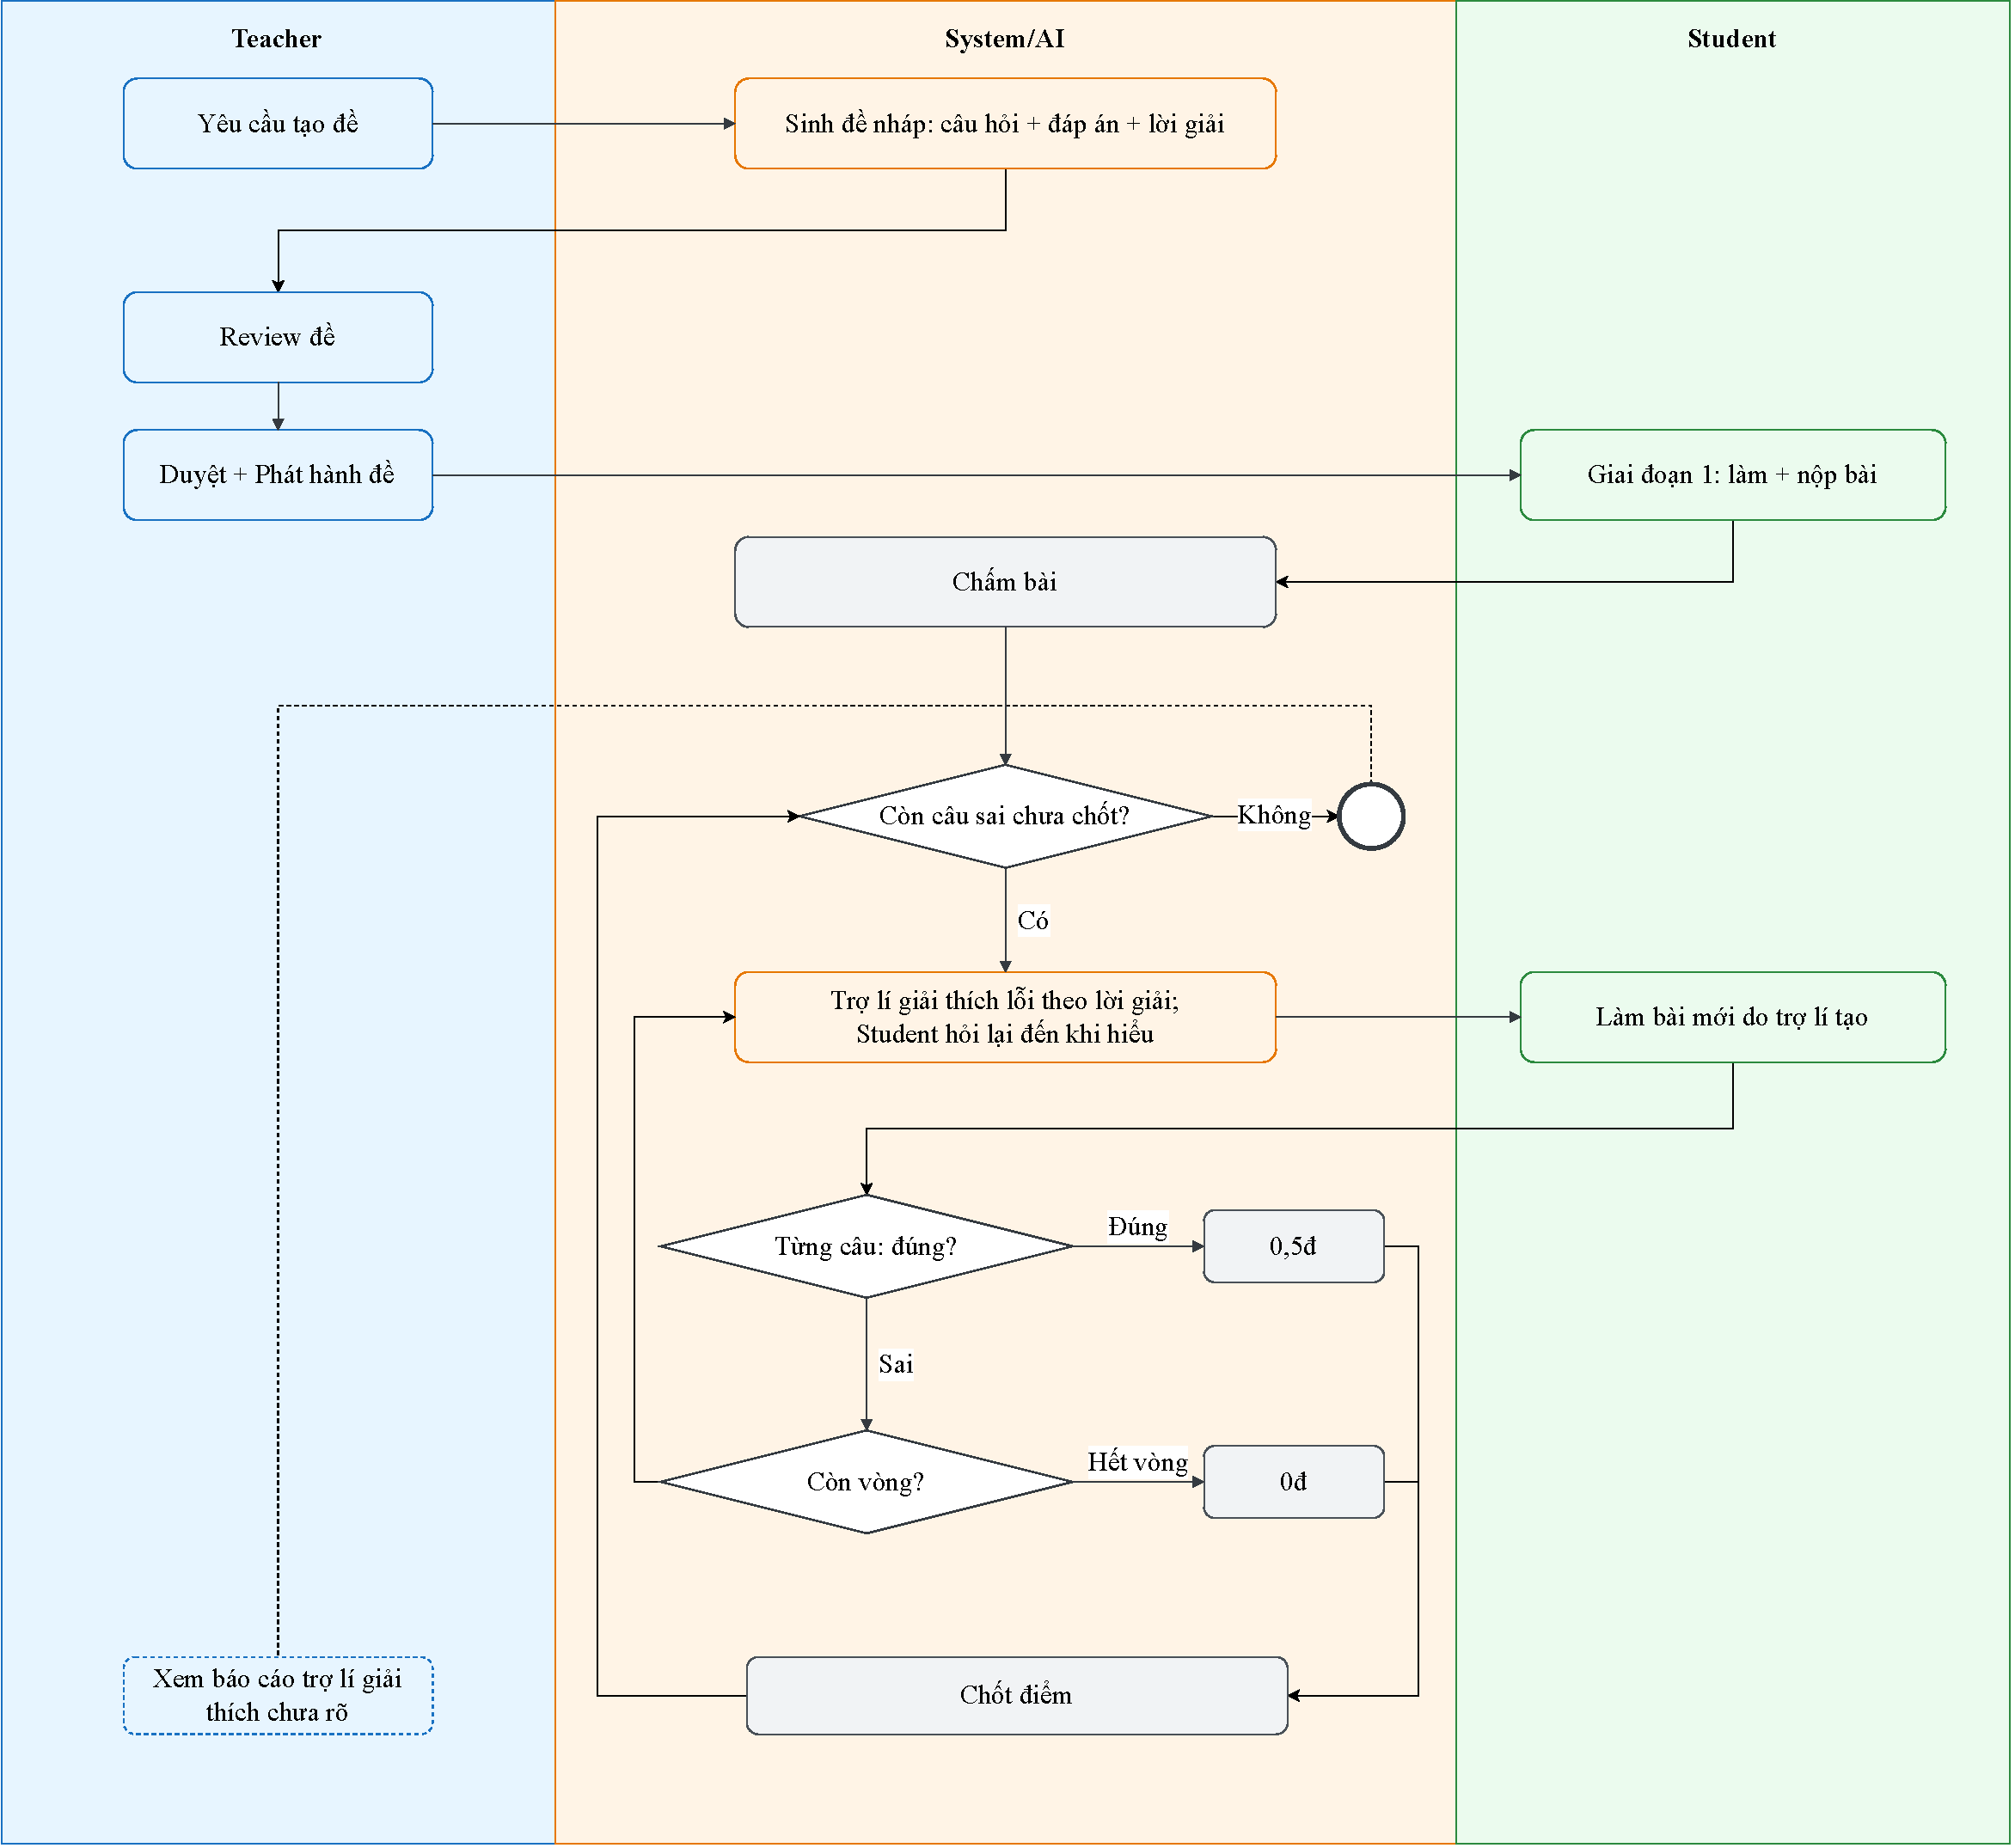
\includegraphics[width=\linewidth,height=\textheight,keepaspectratio]{business-workflows.pdf}
  \caption[Business Workflows]{Business Workflows --- cùng vòng ấy, tách theo lane}
  \label{fig:business-workflows}
\end{figure}
\chapter{Use case}
\label{ch:use-case}

\section{Sáu use case}

\begin{table}[htbp]
\centering
\caption{Sáu use case và actor chính của từng cái}
\label{tab:sau-use-case}
\begin{tabular}{@{}llL{5.4cm}@{}}
\toprule
\textbf{Mã} & \textbf{Actor chính} & \textbf{Tên} \\
\midrule
UC-01 & Teacher & Tạo đề nháp \\
UC-02 & Teacher & Review và phát hành đề \\
UC-03 & Student & Làm và nộp bài (giai đoạn 1) \\
UC-04 & Student & Chữa bài sau khi nộp (giai đoạn 2) \\
UC-05 & --- & Hệ thống tạo câu biến thể \\
UC-06 & Student & Báo cáo chỗ trợ lí giải thích chưa rõ \\
\bottomrule
\end{tabular}
\end{table}

UC-05 không có actor trực tiếp: đó là hành vi hệ thống, được \texttt{<<include>>} từ UC-04.

\begin{landscape}
\begin{figure}[p]
  \centering
  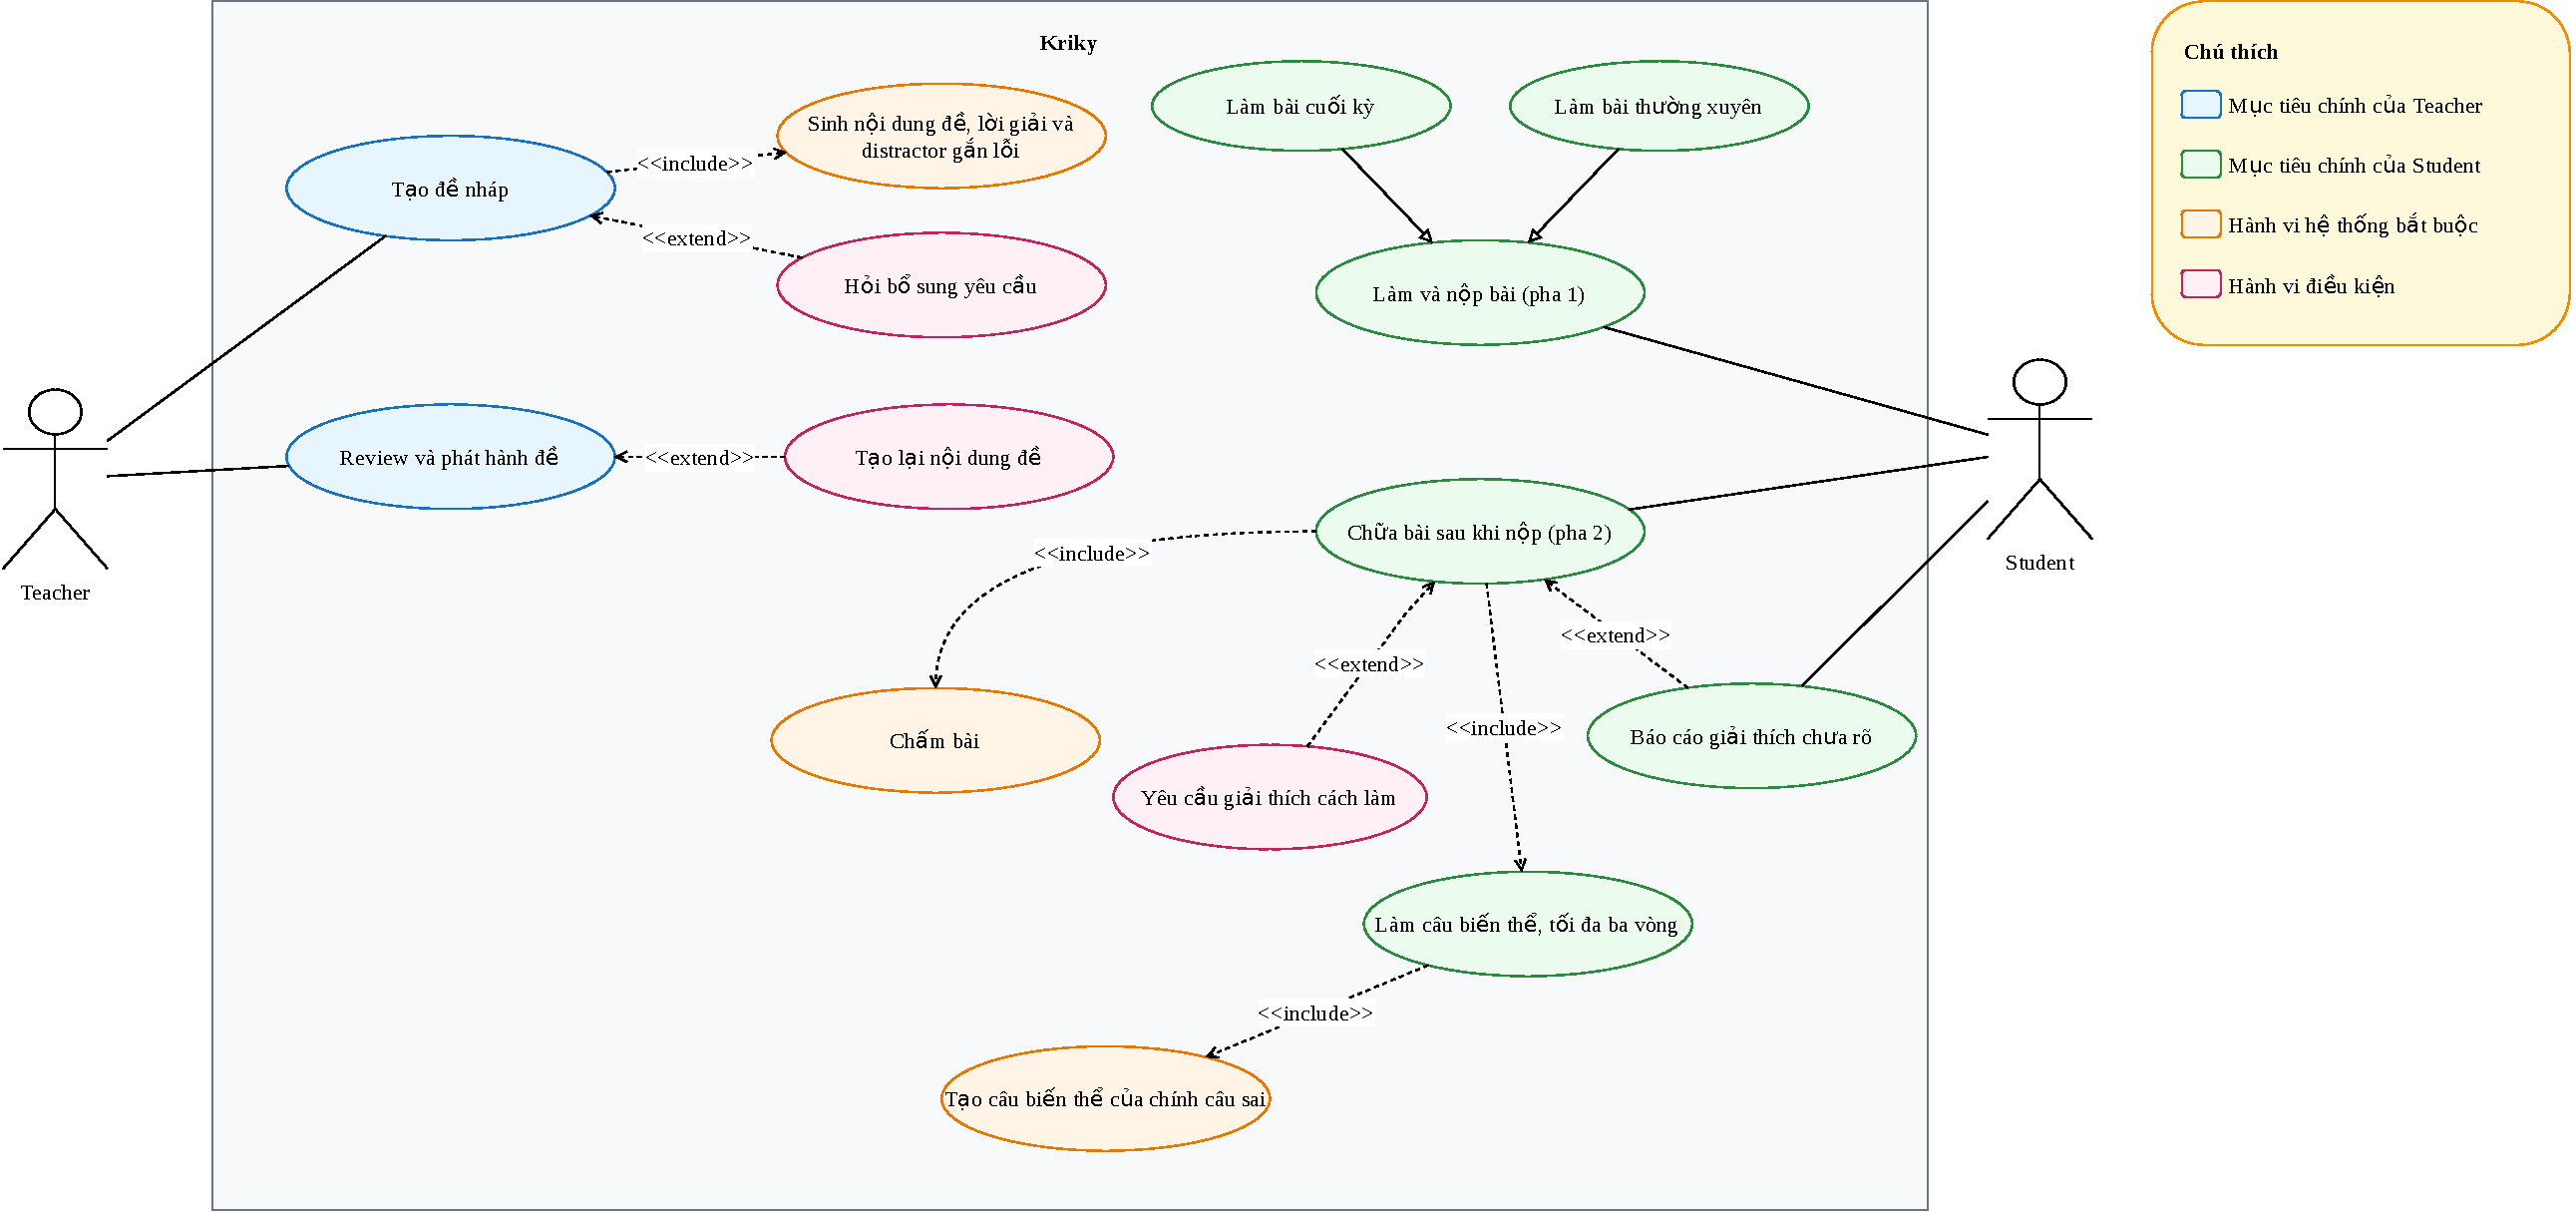
\includegraphics[width=\linewidth,height=\textheight,keepaspectratio]{use-case.pdf}
  \caption[Use Case Diagram]{Use Case Diagram}
  \label{fig:use-case}
\end{figure}
\end{landscape}

\section{Đặc tả từng use case}

\subsection{UC-01 --- Tạo đề nháp}

\paragraph{Điều kiện trước.} Teacher biết chủ đề hoặc mục tiêu học tập cần kiểm tra, và mô tả
được yêu cầu ở mức đủ hiểu.

\paragraph{Luồng chính.} Teacher nhập yêu cầu và các ràng buộc (chủ đề, số câu, độ khó, thời gian
làm bài, loại bài). Hệ thống phân tích, sinh đề nháp gồm câu hỏi, phương án, đáp án đúng, lời giải
và metadata, rồi hiển thị cho Teacher.

\paragraph{Quan hệ.} \emph{Tạo đề nháp} \texttt{<<include>>} \emph{Sinh nội dung đề}. \emph{Hỏi bổ
sung yêu cầu} \texttt{<<extend>>} \emph{Tạo đề nháp}, khi yêu cầu ban đầu chưa đủ rõ --- đây chính
là một trong hai nơi Giáo viên ra quyết định ở mục~\ref{sec:hai-cong}.

\subsection{UC-02 --- Review và phát hành đề}

\paragraph{Điều kiện trước.} Đã có đề nháp.

\paragraph{Luồng chính.} Teacher xem từng câu hỏi, xem đáp án đúng, lời giải và phương án sai;
chỉnh sửa nếu cần; duyệt đề; rồi phát hành với sáu tham số. Mỗi lần phát hành cho một lớp
sinh ra một \emph{Publication}.

\paragraph{Quan hệ.} \emph{Tạo lại nội dung đề} \texttt{<<extend>>} \emph{Review và phát hành đề},
khi Teacher thấy một phần hoặc toàn bộ đề chưa phù hợp.

\subsection{UC-03 --- Làm và nộp bài}

\paragraph{Điều kiện trước.} Bài đã được phát hành và Student có quyền truy cập.

\paragraph{Luồng chính.} Student mở bài, đọc câu hỏi, chọn đáp án, nộp bài. Hệ thống ghi nhận, và chấm bài.

\paragraph{Quan hệ.} \emph{Làm bài thường xuyên} và \emph{Làm bài cuối kỳ} đều generalize lên
\emph{Làm và nộp bài (giai đoạn 1)}.

Sơ đồ \emph{không} dùng \texttt{<<include>>} từ \emph{Làm và nộp bài} sang \emph{Chấm bài}: 
chấm bài là bước xử lý \emph{sau} khi có bài nộp, không phải hành vi bắt buộc để Student hoàn thành mục tiêu nộp bài của mình.

\paragraph{Kết quả.} Bài nộp được ghi nhận và được chấm. \textbf{Nộp bài không kết thúc bài kiểm
tra} --- nó kết thúc giai đoạn 1.

\subsection{UC-04 --- Chữa bài}

\paragraph{Điều kiện trước.} Student đã nộp bài ở giai đoạn 1 và hệ thống đã chấm; chưa quá hạn kết
thúc giai đoạn 2.

\paragraph{Luồng chính.} Student mở kết quả; mở màn hỏi trợ lí, nơi mọi câu sai nằm cùng một màn
và phần giải thích không tính giờ; bấm nút làm bài mới để khởi động đồng hồ của lượt; làm câu biến
thể của từng câu sai. Câu đúng thì chốt 0,5; câu còn sai thì sang vòng tiếp, tối đa ba
vòng, hết ba vòng thì chốt 0.

\paragraph{Ngoại lệ.} Hết hạn giai đoạn 2 giữa một lượt thì lượt bị \emph{dừng} và các câu còn dở nhận
0 điểm. Student không mở giai đoạn 2 lần nào thì mọi câu sai nhận 0 điểm.

\paragraph{Quan hệ.} \emph{Chữa bài} \texttt{<<include>>} \emph{Chấm bài và tra cứu lỗi sai}, và
\texttt{<<include>>} \emph{Làm câu biến thể, tối đa ba vòng}. \emph{Yêu cầu giải thích cách làm}
và \emph{Báo cáo giải thích chưa rõ} đều \texttt{<<extend>>} từ nó.

Quan hệ với \emph{Làm câu biến thể} là \texttt{<<include>>} chứ không phải \texttt{<<extend>>},
\textbf{vì giai đoạn 2 bắt buộc}: nó không phải một nhánh có thể không xảy ra. Đây là ví dụ rõ nhất
trong cả sơ đồ về việc một quyết định sư phạm đổi luôn kiểu quan hệ trên hình.

\subsection{UC-05 --- Tạo câu biến thể}

\paragraph{Điều kiện trước.} Một câu ở giai đoạn 1 bị làm sai.

\paragraph{Luồng chính.} Hệ thống lấy câu Student làm sai, sinh biến thể của \emph{chính câu
đó} --- giữ nguyên cấu trúc và lỗi cần kiểm, thay dữ kiện --- rồi đưa thẳng tới Student. Kết quả của
câu biến thể quyết định câu gốc chốt 0,5 hay sang vòng tiếp.

\subsection{UC-06 --- Báo cáo Trợ lí giải thích chưa rõ}

\paragraph{Điều kiện trước.} Student đang ở giai đoạn 2, và trợ lí đã trả lời ít nhất một lần.

\paragraph{Luồng chính.} Student bấm nút báo cáo ``Trợ lí giải thích chưa rõ''. 
Hệ thống ghi lại \textbf{cả đoạn hội thoại của bài kiểm tra đó} kèm những câu Student
làm sai để giáo viên có thể xem được.

\chapter{Những quyết định nghiệp vụ đáng chú ý}
\label{ch:quyet-dinh}

Những chương trước mô tả hệ thống làm gì. Chương này nói về sáu quyết định mà chọn một đường
là bỏ một đường khác. Cái giá của mỗi lựa chọn đều đã biết trước, chứ không phát hiện ra lúc
dùng.

Mỗi quyết định có ba phần: bối cảnh, quyết định đã chốt, và cái giá đi kèm. Phần thứ ba đáng
đọc nhất, vì một quyết định không mất gì thường là quyết định chưa gặp tình huống khó.

Riêng mục~\ref{sec:hai-luat-nghich} không theo khuôn ấy. Nó không phải quyết định thứ bảy mà là
chỗ hai quyết định trước gặp nhau, và nhìn qua thì chúng mâu thuẫn.

\section{Duyệt khoá nội dung, nhưng bỏ duyệt được}

\paragraph{Bối cảnh.} Mô tả nghiệp vụ ban đầu coi duyệt và phát hành là một bước, nên một đề chỉ
có hai trạng thái: chưa duyệt và đã phát hành. Thiết kế thực tế tách chúng ra, và cần thêm một
trạng thái mà mô hình cũ không có chỗ chứa: đề vừa tạo ra thì chưa có câu nào.

\paragraph{Quyết định.} Một đề đi qua bốn trạng thái: \emph{trống}, \emph{có câu hỏi},
\emph{đã duyệt}, \emph{đã phát hành}. Duyệt \textbf{khoá nội dung} --- ở trạng thái đã duyệt,
không thêm và không sửa câu hỏi được. Nội dung bị khoá gồm cả lời giải và ánh xạ từ phương án
nhiễu sang lỗi, không chỉ câu hỏi và đáp án. Bỏ duyệt đưa đề về lại nháp, và được phép chừng nào
đề chưa phát hành; cài đặt phát hành đã nhập thì giữ nguyên.

Lý do khoá thì dễ thấy: duyệt là lúc giáo viên nhận trách nhiệm về nội dung. Nếu nội dung còn sửa
được sau khi duyệt thì việc duyệt không có nghĩa gì.

Lý do \emph{đảo ngược được} mới là phần đáng nói. Đây không phải cổng cuối cùng --- phát hành
mới là. Nếu cả hai cổng đều một chiều thì giáo viên gặp hai cửa nặng liên tiếp, và sẽ học cách
bấm qua cả hai cho nhanh. Làm nặng cổng duyệt như vậy là làm hỏng đúng cái cổng thật sự cần sức
nặng.

\paragraph{Cái giá.} Giao diện không được mời giáo viên sửa nữa, khi đề đã duyệt. Nút sửa trên từng
câu phải \textbf{biến mất}, không phải mờ đi: một nút mờ vẫn là một lời mời, và chừng nào nó còn
đó thì câu \emph{nội dung đã khoá} chỉ là lời nói suông. Trạng thái trống cũng phải có một màn
hình rỗng riêng và phải chặn phát hành, nên nó là một trạng thái thật chứ không phải một phép
đếm câu hỏi.

\section{Giờ đóng chặn việc vào, không chặn việc nộp}

\paragraph{Bối cảnh.} Mục~\ref{sec:ba-con-so} đã nói luật này và ví dụ đi kèm. Chỗ đáng bàn ở
đây là vì sao nó được chọn, khi mà nó đi ngược với cách hầu hết người đọc hiểu chữ \emph{đóng}.

\paragraph{Quyết định.} Giờ đóng là hạn \textbf{vào tham gia}, không phải hạn nộp. Mốc này bao
gồm chứ không loại trừ: vào tới hết giờ đóng vẫn được. Ai đã vào rồi thì không bị dừng giữa
chừng.

Mốc chọn kiểu bao gồm, vì một học sinh bấm vào đúng giây cuối không nên bị từ chối bởi một ranh
giới em không nhìn thấy. Còn người đã vào thì không bị dừng, vì ở giai đoạn 1 thời gian làm bài
là thứ hệ thống \emph{cấp cho riêng mỗi em}, đo từ lúc em vào. Cắt ngang là lấy lại một thứ đã
hứa.

\paragraph{Cái giá.} Hệ thống nhận lấy nghĩa vụ giải thích. Vì hiểu nhầm ở đây gây hại theo
chiều ngược với dự đoán, câu giải thích phải xuất hiện ở cả ba nơi --- lúc đang chọn giờ, lúc xác
nhận, và trong biên bản sau khi phát hành --- và phải giống hệt nhau từng chữ. Ba cách diễn đạt
cho một luật sẽ được hiểu thành ba luật.

Kéo theo một ràng buộc nữa: mốc nộp cuối trong câu đó --- 18:15 ở ví dụ
mục~\ref{sec:ba-con-so} --- phải được tính từ giờ đóng cộng thời gian làm bài, chứ không viết
sẵn. Viết cứng thì nó sai ngay lần đầu có người đổi thời gian làm bài, và sai một cách im lặng.

\section{Ba cổng, và ranh giới cứng của cổng đầu vào}

\paragraph{Bối cảnh.} Mục~\ref{sec:ba-cong} đã nêu ba điểm giáo viên bắt buộc tham gia. Hai
trong ba nằm ở đầu ra, tức sau khi trợ lí đã làm xong việc. Cổng còn lại nằm ở đầu vào, và nó là
cổng dễ bị lạm dụng nhất.

\paragraph{Quyết định.} Cổng đầu vào --- trợ lí hỏi lại khi chưa đủ thông tin --- có một ranh giới
cứng:

\begin{itemize}
  \item Chỉ dùng để hỏi thông tin \textbf{trước khi làm một việc đảo ngược được}.
  \item \textbf{Không bao giờ} dùng để xin phép một việc không thu hồi được. Câu hỏi
        \emph{phát hành cho lớp nào} phải đi qua biểu mẫu phát hành và hộp xác nhận.
  \item Trợ lí không đánh dấu lựa chọn nào là nên chọn, khi đó là một quyết định sư phạm. Mỗi
        lựa chọn tự nói ra cái giá của nó.
  \item Luôn giữ lối thoát trả lời tự do. Ba lựa chọn không bao giờ phủ hết.
\end{itemize}

Ranh giới cứng còn quan trọng hơn bản thân việc có cổng. Nếu một bộ ba lựa chọn được phép xin
phép một việc không thu hồi được, thì cổng duyệt bị đi vòng bằng một cú bấm --- và nó \emph{sẽ}
bị đi vòng, vì ba cái nút nhẹ hơn hẳn một biểu mẫu sáu trường.

Không đánh dấu nên chọn, vì chọn nguồn câu hỏi hay mức độ khó là quyết định sư phạm. Trợ lí biết
kho câu hỏi còn gì ở mức nào; quyền chọn thì thuộc về giáo viên. Đưa thông tin là đủ, còn nghiêng
người đọc về một phương án là làm thay việc của họ.

\paragraph{Một cái bẫy đã gặp.} Gợi ý ngầm còn tệ hơn gợi ý công khai. Bộ ba lựa chọn soạn lần
đầu có một phương án duy nhất không kèm mệnh đề nhượng bộ, nên nó nghe nhẹ nhất trong ba phương
án, mà người đọc không nhận ra mình đang được hướng về đó. Vì vậy mọi lựa chọn phải nêu cái giá
bằng cùng một ngữ pháp.

\paragraph{Cái giá.} Cổng đầu vào làm trợ lí chậm lại: nó phải nhận ra mình chưa đủ thông tin
thay vì chọn một mặc định hợp lý. Đổi lại, mỗi lần đoán sai đều tốn một vòng sửa ở đầu ra, nơi
đắt hơn.

Và có một lỗ đã biết, ghi ra đây thay vì để nó âm thầm: \textbf{câu biến thể ở giai đoạn 2 không
đi qua cổng nào}. Đây là ngoại lệ của cổng thứ nhất, tức cổng duyệt. Câu biến thể sinh ra lúc học
sinh đang ngồi làm bài, nên không có khoảng trống nào để chờ một thao tác của giáo viên.

Đó là lý do cơ học chứ không phải lý do nguyên tắc: cổng vẫn đúng, chỉ là chưa có cách giữ nó mà
không bắt cả lớp dừng lại. Vì vậy câu \emph{ba cổng} không còn đọc được như một lời hứa tuyệt
đối, và chỗ nào nhắc tới nó cũng phải trả lời được một câu: thế còn câu biến thể?

\section{Hai đồng hồ ở giai đoạn 2, và chỉ một cái chạy khi học sinh đang học}

\paragraph{Bối cảnh.} Giai đoạn 2 cần thời gian, nhưng thời gian của nó không giống giai đoạn 1 ở
bất cứ điểm nào. Số câu phải làm thay đổi theo từng lượt, phần học sinh đọc lời giải thì không
nên bị hối, và cả giai đoạn có thể kéo dài tới cuối ngày.

\paragraph{Quyết định.} Mục~\ref{sec:hai-dong-ho} đã mô tả cơ chế: số phút mỗi câu là một tỉ lệ
chứ không phải một khoảng, thời lượng một lượt là một quỹ chung, phần giải thích không tính giờ,
và đồng hồ chỉ chạy khi học sinh tự bấm nút làm bài mới.

Ba lý do đứng sau ba lựa chọn ấy. Tỉ lệ thay vì khoảng cố định, vì số câu phải chữa giảm dần qua
từng lượt, và một khoảng cố định sẽ quá rộng ở lượt cuối, quá chật ở lượt đầu. Phần giải thích
không tính giờ, vì đó là lúc học sinh đang học chứ không phải lúc em đang chứng minh; đặt đồng hồ
lên một cuộc giải thích chỉ dạy em gật cho xong rồi bấm tiếp. Ranh giới đặt ở nút làm bài mới, vì
đó là hành động do chính em chọn.

\paragraph{Cái giá.} Ba thứ. Hai thứ đổ lên giáo viên, một thứ làm hệ thống mất khả năng đo.

Giáo viên phải đặt một con số mà họ chưa từng phải nghĩ tới. Không có kinh nghiệm dạy học nào
giúp đoán mấy phút là đủ cho một câu chữa, và đặt sai thì hoặc lớp không kịp, hoặc bài kiểm tra
kéo lê.

Số phút mỗi câu là một con số cho cả đề, nên một câu dài và một câu ngắn được cấp thời gian như
nhau. Muốn phân biệt câu dài câu ngắn thì phải thêm một khái niệm khác, chứ không phải tăng con
số này lên.

Và tổng thời gian một học sinh thực sự bỏ ra \textbf{không dự đoán được}, vì phần giải thích
không có giới hạn. Mọi báo cáo sau này muốn nói em học bao lâu đều phải đo, không suy ra được từ
cài đặt phát hành.

\section{Hai luật nghịch nhau, và vì sao đó là chủ ý}
\label{sec:hai-luat-nghich}

Ở giai đoạn 1, học sinh đã vào thì không bị dừng giữa chừng. Ở giai đoạn 2, hết hạn là dừng, kể
cả khi em đang làm dở một lượt, và câu chưa xong nhận 0 điểm. Hai luật này nghịch nhau, và đó là
chỗ dễ bị một người đọc kỹ coi là thiếu nhất quán rồi đi sửa một trong hai.

Chúng không mâu thuẫn, vì thời gian ở hai giai đoạn là hai thứ khác nhau.

Ở giai đoạn 1, thời gian làm bài là một lượng \textbf{hệ thống cấp cho từng người}, bắt đầu đếm
từ lúc em vào. Cắt ngang một người đang làm là lấy lại một thứ đã hứa với riêng em, và em không
có cách nào biết trước mình sẽ bị lấy mất bao nhiêu.

Ở giai đoạn 2 thì ngược hẳn. Thời lượng một lượt do \textbf{học sinh tự chọn lúc nào bắt đầu},
còn hạn kết thúc là một mốc chung cho cả lớp mà em nhìn thấy suốt cả ngày. Không cắt thì hạn ấy
không tồn tại: ai cũng có thể mở một lượt dài lúc chỉ còn một phút, và kéo bài kiểm tra qua đêm.

Cái giá của việc cắt được trả bằng một nghĩa vụ trên giao diện: màn hình phải \textbf{nói trước}
rằng lượt này có thể bị dừng, ngay tại nút làm bài mới, kèm số phút còn lại thật. Một học sinh bị
dừng giữa chừng mà không được báo trước sẽ tin là hệ thống hỏng.

\section{Lời giải nhiều cách, và mỗi phương án nhiễu gắn một lỗi}

\paragraph{Bối cảnh.} Giai đoạn 2 đòi trợ lí giải thích lỗi rồi dạy lại. Muốn làm được, nó phải
biết hai thứ: học sinh sai vì cái gì, và cách làm đúng là gì. Với một hệ thống chỉ có đáp án
đúng trong tay thì nó không biết cả hai, và chỉ còn đường đoán. Mục~\ref{sec:nhan-loi} đã nói vì
sao đoán sai rồi đi giải thích một lỗi học sinh không mắc thì tệ hơn im lặng.

\paragraph{Quyết định.} Mỗi câu hỏi mang theo lời giải có \textbf{nhiều hơn một cách làm}. Mỗi
phương án nhiễu mang theo \textbf{lỗi mà nó đại diện}, soạn cùng câu hỏi chứ không suy ra lúc
chấm. Và trong một câu, không được có hai phương án viết giống nhau từng chữ.

Luật cuối nghe như một chi tiết nhưng không phải. \emph{Đúng một đáp án đúng} là một luật về cái
nhãn đánh dấu đáp án, nên hai phương án trùng chữ vẫn thoả nó. Nhưng với học sinh thì câu đó có
hai đáp án đúng. Em chọn phương án không được đánh dấu sẽ bị chấm là sai, dù em đã chọn đúng.

Giá trị thật của quyết định này là nó biến chẩn đoán từ \textbf{suy đoán} thành \textbf{tra
cứu}, và làm việc đó ở đúng chỗ: lúc soạn đề, nơi có một người biết môn học đang ngồi. Lời giải
nhiều cách thì cần cho một lý do khác --- một cuộc giải thích chỉ có một cách sẽ không đi đâu
được khi học sinh nói em vẫn chưa hiểu, và lặp lại to hơn không phải là dạy.

\paragraph{Cái giá.} Đây là chỗ hệ thống trả giá đắt nhất trong cả báo cáo, và cái giá nằm
đúng vào một nguyên tắc lõi.

Ánh xạ soạn sẵn gắn mỗi phương án nhiễu với đúng một lỗi: chọn nhiễu B thì hệ thống nói ngay là
lỗi B, nói chắc nịch, kể cả khi em chọn B vì một lý do khác hẳn. Đổi lấy sự chắc chắn ấy, sản
phẩm \textbf{mất khả năng nói ra rằng nó không chắc} đúng ở chỗ nó đang nói chuyện với học sinh.

Đánh đổi này được nhận vì phương án còn lại tệ hơn theo cách đo được. Giữ chẩn đoán bằng suy đoán
nghĩa là mọi câu của mọi em đều rơi vào hàng đợi chờ giáo viên, và giai đoạn 2 không khởi động
được cho ai. Một chẩn đoán do người soạn đề viết ra sai ít hơn một chẩn đoán do máy
đoán --- nhưng nó không phải là không sai.

Ba hệ quả đi kèm, và cả ba đều đã biết trước:

\begin{itemize}
  \item \textbf{Cổng duyệt nặng hơn hẳn.} Duyệt một đề nay là duyệt cả lời giải và ánh xạ nhiễu.
        Mà lời giải khó duyệt hơn câu hỏi: một câu hỏi sai thì đọc là thấy, còn một lời giải sai
        tinh vi thì phải làm thử mới thấy.
  \item \textbf{Lời giải sai bị khuếch đại.} Một câu hỏi sai làm hỏng một câu. Một lời giải sai
        được dạy lại cho mọi em sai câu đó, cùng lúc. Sai sót trong nội dung không còn tỉ lệ với
        số người gặp nó.
  \item \textbf{Câu đúng ở giai đoạn 1 không bao giờ kiểm được lời giải của nó}, vì nó không vào
        giai đoạn 2. Một lời giải sai chỉ lộ ra qua chính những em bị dạy lại bằng nó.
\end{itemize}

\section{Đề có tác giả, và câu từ chối phải giống hệt câu không tìm thấy}

\paragraph{Bối cảnh.} Luật \emph{lớp thuộc về giáo viên} đã được phát biểu từ sớm, nhưng chưa
từng có chỗ để sống: dữ liệu không có trường nào ghi ai là tác giả. Không có chỗ ghi thì không
câu truy vấn nào áp được luật, và không phép kiểm nào hỏi được là luật có đúng hay không.

Chuyện này chưa gây hại khi hệ thống chỉ có màn hình của học sinh, vì ở đó phạm vi dữ liệu đã bị
cắt sẵn theo bài làm của chính em. Màn hình của giáo viên phá vỡ điều đó: mọi thứ bắt đầu từ một
cuộc hội thoại, nên trợ lí phải tự chọn dữ liệu để đọc. Câu \emph{trợ lí chỉ đọc được dữ liệu của giáo viên đang đăng
nhập} phải thành một điều kiện trong truy vấn, không phải một dòng trong lời dặn gửi cho mô hình.

\paragraph{Quyết định.} Mỗi lớp và mỗi đề có đúng một tác giả, và trường đó bắt buộc có. Giáo
viên chỉ đọc và chỉ sửa được lớp và đề của mình.

Và phần đáng bàn: \textbf{lớp không tồn tại và lớp của giáo viên khác nhận cùng một câu trả
lời}. Không có mã lỗi riêng, không có câu từ chối riêng, không có chênh lệch nào để so.

Nếu hai câu trả lời ấy khác nhau thì chúng là một kênh dò: gõ tên lớp cho tới khi thông báo đổi
giọng là biết được lớp nào có thật ở trường. Với một trợ lí trò chuyện bằng tiếng Việt thì việc
dò ấy rẻ nhất: người dò không phải đọc mã lỗi, chỉ cần nhận ra hai câu trả lời nghe khác nhau. Mà
sự khác nhau đó thì chính trợ lí sẽ nói ra, rất nhiệt tình.

Đây cũng là lý do luật này là luật nghiệp vụ chứ không phải một chi tiết kỹ thuật: nó nói hệ
thống được phép để lộ điều gì về những người không phải người đang hỏi.

\paragraph{Cái giá.} Câu từ chối mất đi phần hữu ích nhất của nó. Nó \textbf{không được} nói
\emph{đề này không phải của bạn}, vì chính câu đó đã tiết lộ rằng đề tồn tại. Một giáo viên gõ
nhầm tên lớp sẽ nhận một câu trả lời không giúp họ nhận ra mình gõ sai, và đó là cái giá đã biết.

Một tác giả chứ không phải nhiều, cũng là một lựa chọn có giá: đồng sở hữu một đề là chuyện chưa
ai yêu cầu, và nó làm mọi phép kiểm \emph{đề này của ai} nặng thêm một bậc. Thêm vào sau thì
được; bỏ đi thì không.

\paragraph{Và tên lớp không phải định danh.} Hai lớp cùng tên được phép tồn tại, nên khi giáo
viên nhắc tới một cái tên mà có nhiều lớp mang tên đó, trợ lí phải hỏi lại chứ không được tự
chọn. Đó chính là cổng đầu vào ở mục~\ref{sec:ba-cong} làm việc đúng chỗ của nó.

% Chương này được viết ở một task sau. Hiện chỉ có tiêu đề để khung build được.
\chapter{Kiến trúc và mô hình dữ liệu}
\label{ch:kien-truc-va-du-lieu}


\end{document}
